\chapter{Result}
 This chapter consists of two parts: experiment results and comparison. All experiment results are in the first part, and the comparisons of different experiment data are in the second part. To observe the patch-based and patient-based AUC performance on target data, 10-folder cross-validation is applied to validate all the experiments.

\section{Basic Models}
\subsection{Train Models Using Only Source Data (B1)}
This experiment is applied to validate that how much AUC performance other algorithms improve. Only source data is applied for model training. 

Ten-folder cross-validation was performed 3 times to get three sets of source data models. Figure 4.1 and figure 4.2 show the patch-based and patient-based AUC performance of experiment B1, respectively. The patch-based AUC performance on target data varied from 0.71 to 0.84 while the patient-based AUC performance varied from 0.58 to 0.98. The AUC value of source data model will heavily influence the experiment results on transfer learning or incremental learning. \\

\begin{figure}[H]
    \hfil
    \begin{minipage}[t]{0.9\textwidth}
        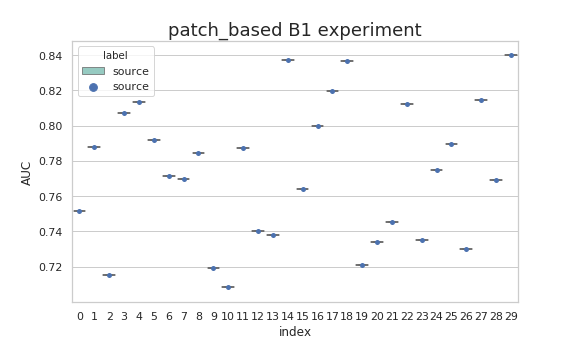
\includegraphics[width=\textwidth]{fig/B1_index_patch.png}
        \caption{\label{fig:parallel1} Patch-based AUC for B1 Experiment (different folder)}
    \end{minipage}
    \hfil
\end{figure}
\begin{figure}[H]
    \hfil
    \begin{minipage}[t]{0.9\textwidth}
        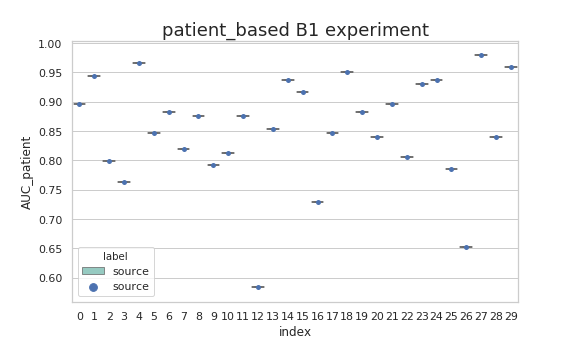
\includegraphics[width=\textwidth]{fig/B1_index_patient.png}
        \caption{\label{fig:parallel1} Patient-based AUC for B1 Experiment (different folder)}
    \end{minipage}
    \hfil
\end{figure}
\subsection{Train Models Using Only Target Data (B2)}
This experiment is applied to validate that how much target data is needed to get a workable classification model. Only target data is applied for model training. 

Ten-folder cross-validation was performed to get 10 target data models. Figure 4.3 and figure 4.4 show the patch-based and patient-based AUC performance of experiment B2, respectively. 
Building a model using only target data under 120 is hard to get a accurate model, and the AUC performance increases as the number of target data increases. If the number of training data is higher than 200, both patch-based and patient-based result is more stable.
\begin{figure}[H]
    \hfil
    \begin{minipage}[t]{0.9\textwidth}
        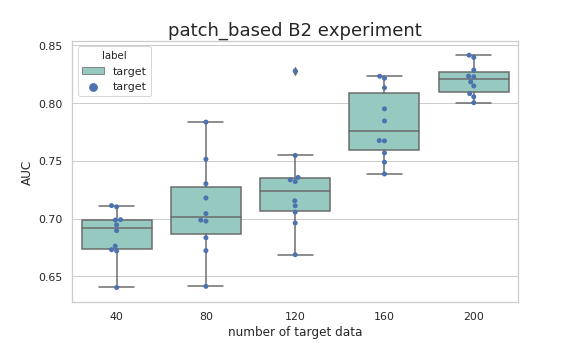
\includegraphics[width=\textwidth]{fig/B2_num_patch.png}
        \caption{\label{fig:parallel1} Patch-based AUC for B2 Experiment}
    \end{minipage}
    \hfil
\end{figure}
\begin{figure}[H]
    \hfil
    \begin{minipage}[t]{0.9\textwidth}
        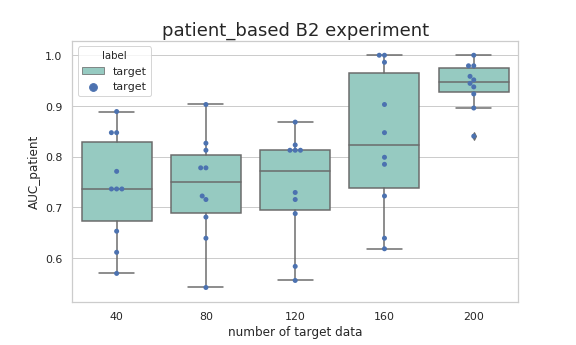
\includegraphics[width=\textwidth]{fig/B2_num_patient.png}
        \caption{\label{fig:parallel1} Patient-based AUC for B2 Experiment}
    \end{minipage}
    \hfil
\end{figure}

\subsection{Choose the Number of Fixed Layers in Fine-tuning Experiments (B3)}
This experiment is applied to choose the number of fixed layers. Fine-tuning is an efficient method to improve the AUC performance on target data. Therefore choosing the number of layers fixed is an important issue for further experiments.

Ten-folder cross-validation was performed to get 10 fine-tuning data models. Figure 4.5 and figure 4.6 show the patch-based and patient-based AUC performance of experiment B3, respectively. Two hundred target data is applied in this experiment. Models fixing no layers or models fixing the first three layers have the highest AUC. However, fixing the first three layers needs less calculation time, so I choose to fix the first three layers in fine-tuning and incremental learning experiments. 
\begin{figure}[H]
    \hfil
    \begin{minipage}[t]{0.9\textwidth}
        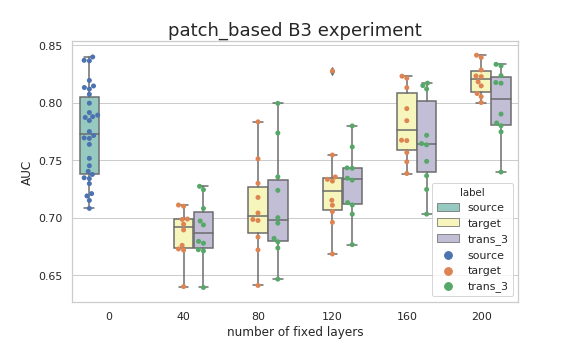
\includegraphics[width=\textwidth]{fig/B3_num_patch.png}
        \caption{\label{fig:parallel1}Patch-based AUC for B3 Experiment}
    \end{minipage}
    \hfil
\end{figure}
\begin{figure}[H]
    \hfil
    \begin{minipage}[t]{0.9\textwidth}
        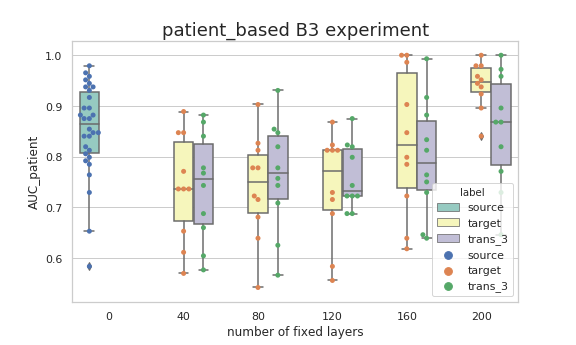
\includegraphics[width=\textwidth]{fig/B3_num_patient.png}
        \caption{\label{fig:parallel1} Patient-based AUC for B3 Experiment}
    \end{minipage}
    \hfil
\end{figure}

~\\
\section{Mixed Data Models}
\subsection{Mixed Data Models (M1)}
This experiment shows the simplest way to improve model AUC using source dataset. In this experiment, I mixed source dataset and target dataset and set this new dataset as the training set. 

Ten-folder cross-validation was performed to get 10 mixed data models. Figure 4.7 and figure 4.8 show the patch-based and patient-based AUC performance of experiment M1, respectively. 

In this experiment, the AUC increases as the number of target data increases. Although this experiment actually improves the AUC performance, it takes too much time on training since is the training set composed of both source and target dataset.

\begin{figure}[H]
    \hfil
    \begin{minipage}[t]{0.9\textwidth}
        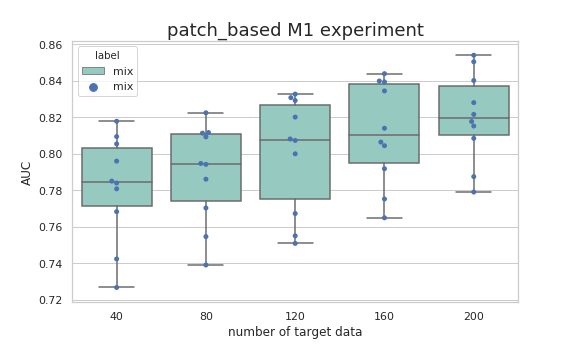
\includegraphics[width=\textwidth]{fig/M1_num_patch.png}
        \caption{\label{fig:parallel1}Patch-based AUC for M1 Experiment}
    \end{minipage}
    \hfil
\end{figure}
\begin{figure}[H]
    \hfil
    \begin{minipage}[t]{0.9\textwidth}
        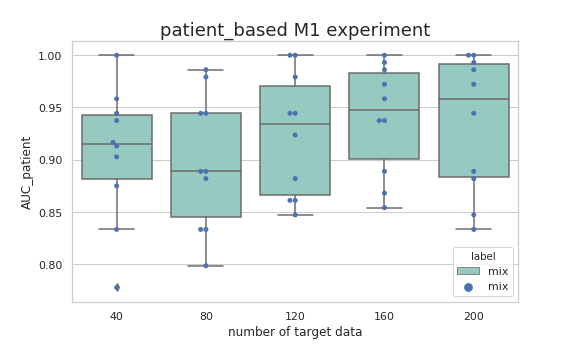
\includegraphics[width=\textwidth]{fig/M1_num_patient.png}
        \caption{\label{fig:parallel1}Patient-based AUC for M1 Experiment}
    \end{minipage}
    \hfil
\end{figure}
~\\
\section{Fine-Tuning Models}
\subsection{Fine-Tuning Models (F1)}
Fine-tuning, a kind of transfer learning method, is applied in this experiment to increase AUC of source data model (B1). The first three layers are fixed in this experiment based on the result of experiment B3.

Ten-folder cross-validation was performed to get 10 mixed data models. Figure 4.9 and figure 4.10 show the patch-based and patient-based AUC performance of experiment F1, respectively. 

In this experiment, the AUC increases as the number of target data increases. It takes less time on training compared to experiment M1 since is the training set (for fine tuning) composed of only target dataset.

\begin{figure}[H]
    \hfil
    \begin{minipage}[t]{0.9\textwidth}
        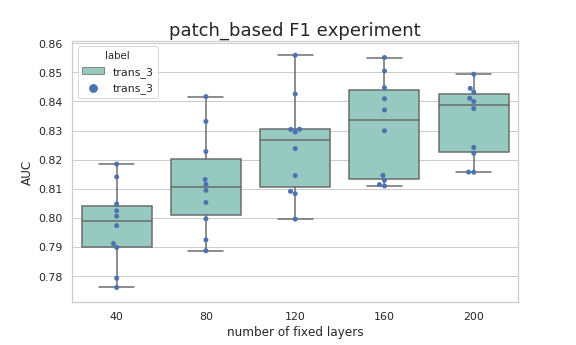
\includegraphics[width=\textwidth]{fig/F1_num_patch.png}
        \caption{\label{fig:parallel1}Patch-based AUC for F1 Experiment}
    \end{minipage}
    \hfil
\end{figure}
\begin{figure}[H]
    \hfil
    \begin{minipage}[t]{0.9\textwidth}
        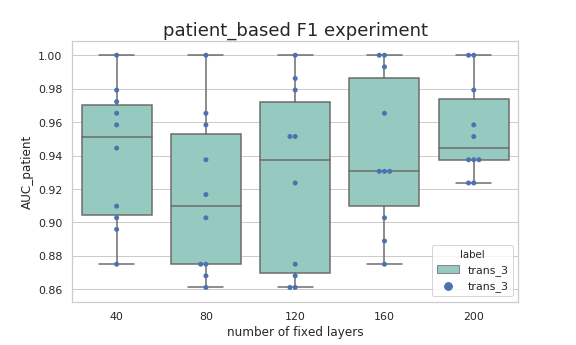
\includegraphics[width=\textwidth]{fig/F1_num_patient.png}
        \caption{\label{fig:parallel1} Patient-based AUC for F1 Experiment}
    \end{minipage}
    \hfil
\end{figure}
~\\
\section{Incremental Fine-Tuning Models}
In this part, I test the algorithm in thesis \cite{zhou2017fine} on pancreatic images to validate the algorithm performance. 
\subsection{Fine-tuning Using Selected/Random Target Data (S1/R1)}
This experiment is applied to observe the AUC performance and validate if the selection method AIFT works compared to random selection. Forty patient data is selected in each selection step. Since the difference among two selection method is highly empathized in the experiment, we use 200 epochs to run each selection steps to make sure that the training process won't stop too early. 

Ten-folder cross-validation was performed twice to get 20 mixed data models since the AUC results are not clear enough.
Figure 4.11, figure 4.12, figure 4.13 and figure 4.14 show the patch-based or patient-based AUC performance of experiment F1. 

In this experiment, the AUC increases as the number of target data increases. The AUC increase heavily compared to normal fine-tuning model, but increase slowly after the first selection step.

\begin{figure}[H]
    \hfil
    \begin{minipage}[t]{0.9\textwidth}
        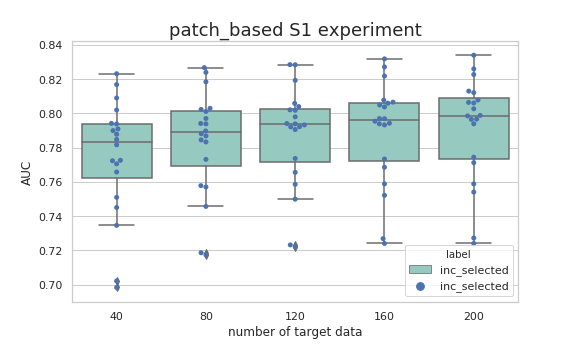
\includegraphics[width=\textwidth]{fig/S1_num_patch.png}
        \caption{\label{fig:parallel1}Patch-based AUC for S1 Experiment}
    \end{minipage}
    \hfil
\end{figure}
\begin{figure}[H]
    \hfil
    \begin{minipage}[t]{0.9\textwidth}
        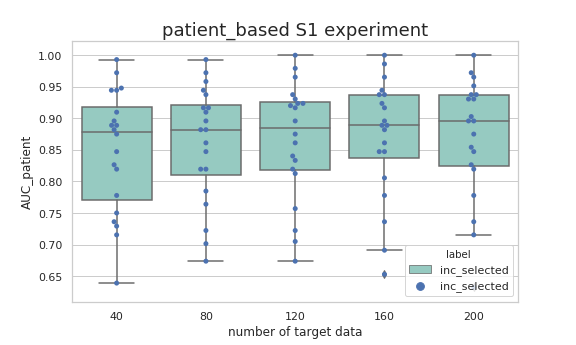
\includegraphics[width=\textwidth]{fig/S1_num_patient.png}
        \caption{\label{fig:parallel1}Patient-based AUC for S1 Experiment}
    \end{minipage}
    \hfil
\end{figure}
~\\
\begin{figure}[H]
    \hfil
    \begin{minipage}[t]{0.9\textwidth}
        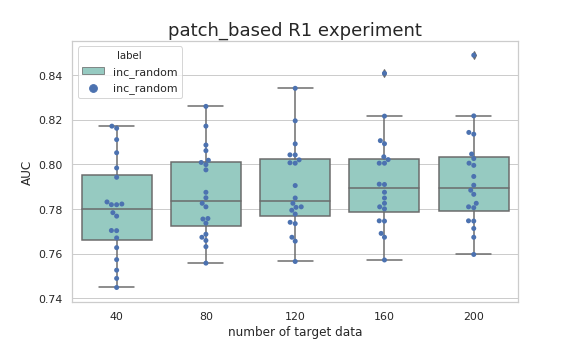
\includegraphics[width=\textwidth]{fig/R1_num_patch.png}
        \caption{\label{fig:parallel1}Patch-based AUC for R1 Experiment}
    \end{minipage}
    \hfil
\end{figure}
\begin{figure}[H]
    \hfil
    \begin{minipage}[t]{0.9\textwidth}
        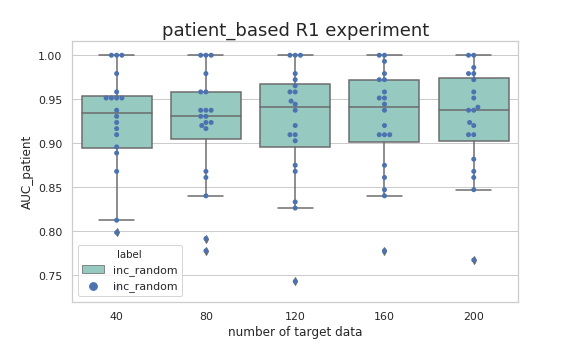
\includegraphics[width=\textwidth]{fig/R1_num_patient.png}
        \caption{\label{fig:parallel1}Patient-based AUC for R1 Experiment}
    \end{minipage}
    \hfil
\end{figure}
~\\
\subsection{Number of Target Data in each Selection Step (S2/R2)}

This experiment is applied to observe the AUC performance of incremental learning model with different selection steps. 

Ten-folder cross-validation was performed to get 10 mixed data models.
Figure 4.15, Figure 4.16, Figure 4.17 and figure 4.18 show the patch-based or patient-based AUC performance of experiment F1. 

In this experiment, the AUC increases as selection step increases. The AUC increase heavily when selection step is less than 60. The AUC performance is not stable in random selection experiments.

\begin{figure}[H]
    \hfil
    \begin{minipage}[t]{0.9\textwidth}
        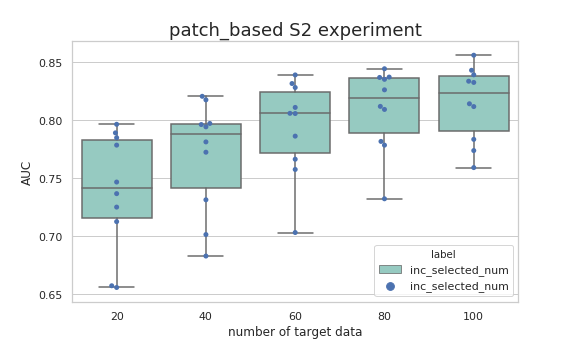
\includegraphics[width=\textwidth]{fig/S2_num_patch.png}
        \caption{\label{fig:parallel1}Patch-based AUC for S2 Experiment}
    \end{minipage}
    \hfil
\end{figure}
\begin{figure}[H]
    \hfil
    \begin{minipage}[t]{0.9\textwidth}
        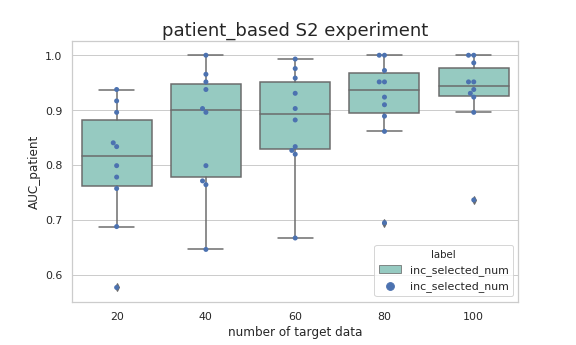
\includegraphics[width=\textwidth]{fig/S2_num_patient.png}
        \caption{\label{fig:parallel1}Patient-based AUC for S2 Experiment}
    \end{minipage}
    \hfil
\end{figure}
~\\
\begin{figure}[H]
    \hfil
    \begin{minipage}[t]{0.9\textwidth}
        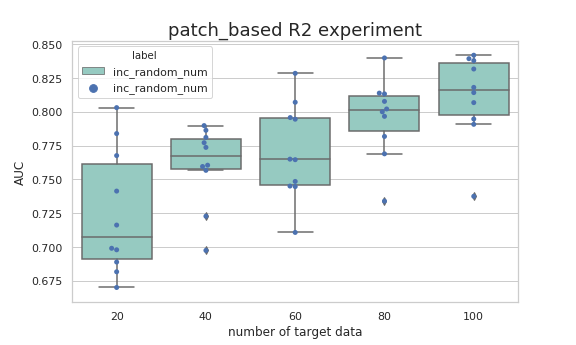
\includegraphics[width=\textwidth]{fig/R2_num_patch.png}
        \caption{\label{fig:parallel1} Patch-based AUC for R2 Experiment}
    \end{minipage}
    \hfil
\end{figure}
\begin{figure}[H]
    \hfil
    \begin{minipage}[t]{0.9\textwidth}
        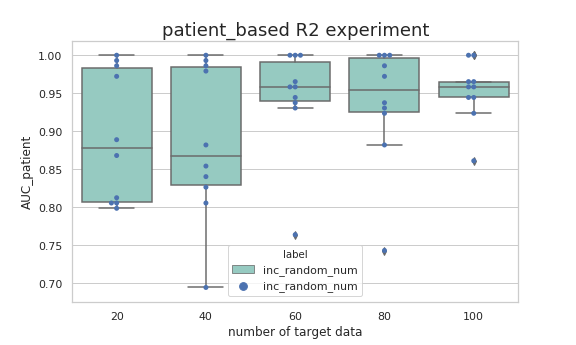
\includegraphics[width=\textwidth]{fig/R2_num_patient.png}
        \caption{\label{fig:parallel1}Patient-based AUC for R2 Experiment}
    \end{minipage}
    \hfil
\end{figure}
~\\

\subsection{Reduce the Epochs to Compare With Fine-tuning Experiments (S3/R3)}
This experiment is applied to observe the AUC performance of incremental learning model if both calculation waste are the same. Two hundred epochs is set for normal fine-tuning model (number of target data is 200), and 66 epochs is set for incremental learning (number of target data varies from 40 to 200). 

Ten-folder cross-validation was performed to get 10 mixed data models.
Figure 4.19, Figure 4.20, Figure 4.21 and figure 4.22 show the patch-based or patient-based AUC performance of experiment S3/R3. 

In this experiment, the AUC increases as target data increases.


\begin{figure}[H]
    \hfil
    \begin{minipage}[t]{0.9\textwidth}
        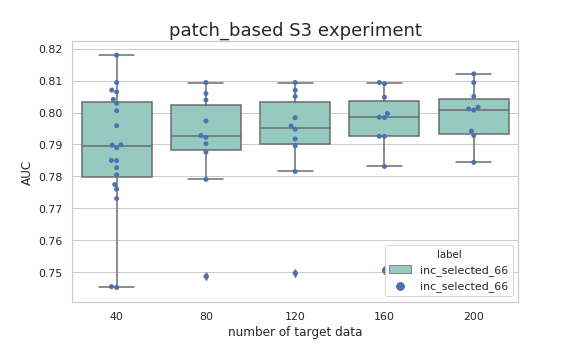
\includegraphics[width=\textwidth]{fig/S3_num_patch.png}
        \caption{\label{fig:parallel1}Patch-based AUC for S3 Experiment}
    \end{minipage}
    \hfil
\end{figure}
\begin{figure}[H]
    \hfil
    \begin{minipage}[t]{0.9\textwidth}
        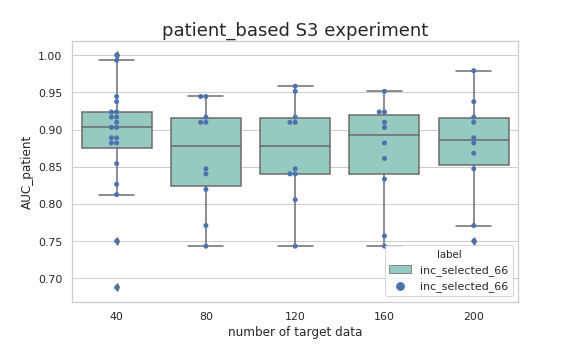
\includegraphics[width=\textwidth]{fig/S3_num_patient.png}
        \caption{\label{fig:parallel1}Patient-based AUC for S3 Experiment}
    \end{minipage}
    \hfil
\end{figure}
~\\
\begin{figure}[H]
    \hfil
    \begin{minipage}[t]{0.9\textwidth}
        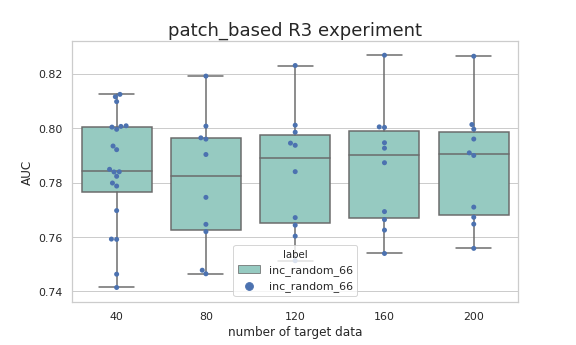
\includegraphics[width=\textwidth]{fig/R3_num_patch.png}
        \caption{\label{fig:parallel1}Patch-based AUC for R3 Experiment}
    \end{minipage}
    \hfil
\end{figure}
\begin{figure}[H]
    \hfil
    \begin{minipage}[t]{0.9\textwidth}
        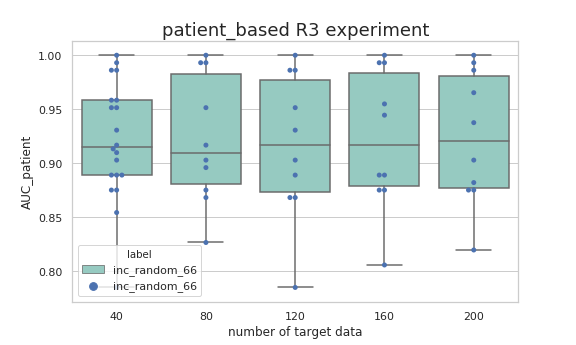
\includegraphics[width=\textwidth]{fig/R3_num_patient.png}
        \caption{\label{fig:parallel1}Patient-based AUC for R3 Experiment}
    \end{minipage}
    \hfil
\end{figure}
~\\

